\documentclass{article}
\title{CP-ALS-QR report}
\author{Alex Zhang}
\date{July 2023}
\textwidth=16.00cm 
\textheight=22.00cm 
\topmargin=0.00cm
\oddsidemargin=0.00cm 
\evensidemargin=0.00cm 
\headheight=0cm 
\headsep=0.5cm
\textheight=610pt
\usepackage{graphicx}
\usepackage{lineno,hyperref}
\usepackage{amsmath,amssymb,enumerate,graphicx,pifont,color,tikz,yfonts,scalerel,changepage,algorithm,algpseudocode}
\usepackage{bookmark}
\usepackage{diagbox}
\usepackage{caption,subcaption}

\usetikzlibrary{positioning}
\usetikzlibrary{cd}

\usepackage{booktabs}
\usepackage{multirow}
\usepackage{tabularx}
\usepackage{array}
\usepackage{tikz}
\usepackage{cleveref}


\graphicspath{{fig/}}

\usepackage{latexsym,array,delarray,amsthm,amssymb,epsfig}
\usepackage{amsmath}
\usepackage{listings}
\lstset{
  basicstyle=\ttfamily,
  mathescape
}

\newcommand{\bmat}[1]{\begin{bmatrix} #1 \end{bmatrix}}
\newcommand{\mat}[1]{\mathbf{#1}}
\newcommand{\ten}[1]{\mathcal{#1}}
% matrix/vector/tensor/element macros
\usepackage{bm}
\newcommand{\Tra}{T}										% transpose
\newcommand{\M}[2][]{\bm{#1{\mathbf{\MakeUppercase{#2}}}}} 		% matrix
\newcommand{\Me}[3][]{\bm{#1{\mathbf{\MakeUppercase{#2}}}}({#3})} 		% matrix entry
\newcommand{\Mb}[3][]{\bm{#1{\mathbf{\MakeUppercase{#2}}}}_{#3}}       	% submatrix
\newcommand{\Mbe}[4][]{\bm{#1{\mathbf{\MakeUppercase{#2}}}}_{#3}({#4})}	% submatrix entry
\newcommand{\Ms}[3][]{\bm{#1{\mathbf{\MakeUppercase{#2}}}}^{(#3)}}       	% matrix in series
\newcommand{\Mbs}[4][]{\bm{#1{\mathbf{\MakeUppercase{#2}}}}_{#3}^{(#4)}}   % submatrix in series
\newcommand{\V}[2][]{\bm{#1{\mathbf{\MakeLowercase{#2}}}}} 		% vector
\newcommand{\Vs}[3][]{\bm{#1{\mathbf{\MakeLowercase{#2}}}}^{(#3)}} 		% vector in series
\newcommand{\Ve}[3][]{\bm{#1{\mathbf{\MakeLowercase{#2}}}}({#3})}		% vector entry
\newcommand{\T}[2][]{#1{\mathbf{\cal{#2}}}} 						% tensor
\newcommand{\Te}[3][]{#1{\mathbf{\cal{#2}}}({#3})}		

\let\ds\displaystyle

\newcommand{\GB}[1]{\textcolor{red}{\textbf{GB}: #1}}


\begin{document}



\maketitle
\section{Introduction}
%The CANDECOMP/PARAFAC or canonical polyadic (CP) decomposition for multidimensional data, 
%or tensors, is a popular tool for analyzing and interpreting latent patterns that may be 
%present in multidimensional data. Basically CP decomposition of a tensor refers to its
%expression as a sum of $r$ rank-one components and each of them is a vector outer product.
%One of the most popular methods used to compute a CP decomposition is the alternating least
%squares (CP-ALS) approach, which solves a series of linear least squares problems. Usually
%to solve these linear leaste squares problems, normal equations are used for CP-ALS. This
%approach may be sensitive for ill-conditioned inputs. Based on this idea, there are already
%a more stable approach which is solving the linear least sqaures problems using QR decomposition
%instead.

%For my summer research project, I basically follows the QR apprach but trying to 
%improve the efficiency for QR decomposition when assuming the input tensor is in Kruskal structure,
%that is, a tensor stored as factor matrices and corresponding weights. By exploiting this structure, 
%we improve the computation efficiency by not forming Multi-TTM tensor.
%The problem left is when doing CP-ALS, QR-based methods is exponential in $N$, the number of modes.
%The normal equations approach is linear in $N$ for Kruskal tensor. During the summer I tried
%to revise and implement former QR method which archieved better stability than normal equations
%but computation time increases linearly with respect to $N$.
copy this senctence till everything is in right position\\
copy this senctence till everything is in right position\\
copy this senctence till everything is in right position\\
copy this senctence till everything is in right position\\
copy this senctence till everything is in right position\\
copy this senctence till everything is in right position\\
copy this senctence till everything is in right position\\
copy this senctence till everything is in right position\\
copy this senctence till everything is in right position\\
copy this senctence till everything is in right position\\
copy this senctence till everything is in right position\\
copy this senctence till everything is in right position\\
copy this senctence till everything is in right position\\
copy this senctence till everything is in right position\\
copy this senctence till everything is in right position\\
copy this senctence till everything is in right position\\
copy this senctence till everything is in right position\\
copy this senctence till everything is in right position\\
copy this senctence till everything is in right position\\
copy this senctence till everything is in right position\\









\section{Background}
\subsection{CP Decomposition}
Given a $d$-way tensor $\T{X} \in \mathbb{R}^{n_1\times n_2\times \dots \times n_d}$, its
CP decomposition of rank $r \in \mathbb{N}$ can be represented as 
$$\T{X}(i_1,i_2,\dots, i_d) \approx \sum^{r}_{j=1}\mat{A_1}(i_1,j)\mat{A_2}(i_2,j) \dots \mat{A_r}(i_r,j)$$
$$\text{for all } (i_1,i_2,\dots, i_d) \in [n_1] \otimes [n_2] \otimes [n_3] \otimes \dots \otimes [n_d]$$
where $\mat{A_k} \in \mathbb{R}^{n_k \times r}$ is a factor matrix for all $k \in [d]$. 
There is a visualization of a CP Decomposition for a 3-way tensor in \cref{fig:3d-cp-decomp}.

\begin{figure}[ht!]
\centering
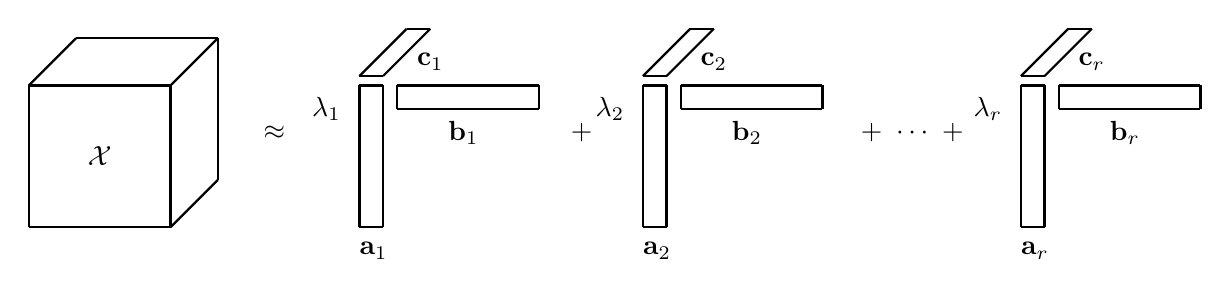
\begin{tikzpicture}[scale=0.6]
%\draw[step=1cm,gray,very thin] (0,0) grid (28,6); %grid lines

\draw node (X) at (1.5, 2.5) {$\T{X}$};
\draw[thick] (0,1) -- (3,1);
\draw[thick] (0,1) -- (0,4);
\draw[thick] (0,4) -- (3,4);
\draw[thick] (3,4) -- (3,1);
\draw[thick] (0,4) -- (1,5);
\draw[thick] (1,5) -- (4,5);
\draw[thick] (3,4) -- (4,5);
\draw[thick] (4,5) -- (4,2);
\draw[thick] (4,2) -- (3,1);

\draw node at (5.2, 3) {$\approx$};

\draw node at (6.3, 3.5) {$\lambda_1$};

\draw node at (7.3, 0.5) {$\V{a}_1$};
\draw[thick] (7,1) -- (7.5,1);
\draw[thick] (7,1) -- (7,4);
\draw[thick] (7,4) -- (7.5,4);
\draw[thick] (7.5,1) -- (7.5,4);

\draw node at (9.2, 3) {$\V{b}_1$};
\draw[thick] (7.8,3.5) -- (7.8,4);
\draw[thick] (7.8,3.5) -- (10.8,3.5);
\draw[thick] (7.8,4) -- (10.8,4);
\draw[thick] (10.8,4) -- (10.8,3.5);

\draw node at (8.5, 4.5) {$\V{c}_1$};
\draw[thick] (7,4.2) -- (7.5,4.2);
\draw[thick] (7,4.2) -- (8,5.2);
\draw[thick] (8,5.2) -- (8.5,5.2);
\draw[thick] (7.5,4.2) -- (8.5,5.2);

\draw node at (11.7, 3) {$+$};

\draw node at (12.3, 3.5) {$\lambda_2$};

\draw node at (13.3, 0.5) {$\V{a}_2$};
\draw[thick] (13,1) -- (13.5,1);
\draw[thick] (13,1) -- (13,4);
\draw[thick] (13,4) -- (13.5,4);
\draw[thick] (13.5,1) -- (13.5,4);

\draw node at (15.2, 3) {$\V{b}_2$};
\draw[thick] (13.8,3.5) -- (13.8,4);
\draw[thick] (13.8,3.5) -- (16.8,3.5);
\draw[thick] (13.8,4) -- (16.8,4);
\draw[thick] (16.8,4) -- (16.8,3.5);

\draw node at (14.5, 4.5) {$\V{c}_2$};
\draw[thick] (13,4.2) -- (13.5,4.2);
\draw[thick] (13,4.2) -- (14,5.2);
\draw[thick] (14,5.2) -- (14.5,5.2);
\draw[thick] (13.5,4.2) -- (14.5,5.2);

\draw node at (18.7, 3) {$+ \ \cdots \ +$};

\draw node at (20.3, 3.5) {$\lambda_r$};

\draw node at (21.3, 0.5) {$\V{a}_r$};
\draw[thick] (21,1) -- (21.5,1);
\draw[thick] (21,1) -- (21,4);
\draw[thick] (21,4) -- (21.5,4);
\draw[thick] (21.5,1) -- (21.5,4);

\draw node at (23.2, 3) {$\V{b}_r$};
\draw[thick] (21.8,3.5) -- (21.8,4);
\draw[thick] (21.8,3.5) -- (24.8,3.5);
\draw[thick] (21.8,4) -- (24.8,4);
\draw[thick] (24.8,4) -- (24.8,3.5);

\draw node at (22.5, 4.5) {$\V{c}_r$};
\draw[thick] (21,4.2) -- (21.5,4.2);
\draw[thick] (21,4.2) -- (22,5.2);
\draw[thick] (22,5.2) -- (22.5,5.2);
\draw[thick] (21.5,4.2) -- (22.5,5.2);
\end{tikzpicture}


\caption{CP decomposition of rank $R$ for a three-dimensional tensor $\T{X}$ \label{fig:3d-cp-decomp}}
\end{figure}

\subsection{Linear Least Square Problem}
In mathematical form, a generic least squares problem is given by 
$$\min_{\mat{X}}||\mat{B} - \mat{X}\mat{A}^\top||_{F}.$$
Note that the coefficient matrix $\mat{A}$ appears on the right of the variable matrix, which is the opposite of the standard form.
We use this form to relate to the corresponding least squares problem that arises in the context of the CP decomposition.

Several different techniques can be used to solve this problem.
The two we consider here are via the Normal Equations and by QR decomposition.
For normal equation, we take the gram of $\mat{A}$ and then compute $\mat{A}^\top\mat{B}^\top$. In sample equation we perform
\begin{align}
\mat{X}\mat{A}^\top\mat{A} &= \mat{B}\mat{A} \nonumber \\
\mat{A}^\top\mat{A}\mat{X}^\top &= \mat{A}^\top\mat{B}^\top \nonumber \\
\mat{X}^\top &= (\M{A}^\top\mat{A})^{-1}\mat{A}^\top\mat{B}^\top \nonumber
\end{align}
Which the time complexity for using normal equation will be $O(n^3)$, given $\mat{A} \in \mathbb{R}^{n \times n}$.

For QR factorization, we will first compute QR decomposition for matrix $\mat{A} = \mat{Q}\mat{R}$ and then apply inverse of $\mat{R}$. In term
of sample problem, we will do
\begin{align}
  \mat{X}\mat{A}^\top &= \mat{B} \nonumber \\
  \mat{X}(\mat{Q}\mat{R})^\top &= \mat{B} \nonumber \\
  \mat{X}\mat{R}^\top\mat{Q}^\top\mat{Q} &= \mat{B}\mat{Q} \nonumber \\
  \mat{X}^\top &= \mat{R}^{-\top}\mat{B}\mat{Q} \nonumber
\end{align} 
The time complexity for solving least square problem with QR factorization will be $O(n^3)$.


If $\mat{B}$ has few columns, using normal equation will be better because of smaller coeffieicnt
for leading polynomial. However, when $\mat{B}$ is really wide, the majority cost 
is computing $\mat{A}^\top\mat{B}^\top$ for normal equation and $\mat{B}\mat{Q}$ for QR factorization, 
which makes the execution time equivalent.
When $\mat{B}$ is large, numerically speaking, using QR decomposition method is more preferred because this method is stable
and not sensitive to rounding errors.







\subsection{CP-ALS}
In terms of the work in CP-ALS, we need to solve bunch of least square problems in the form 
$$\min_{\mat{\hat{A}}_n}||\mat{X_{(n)}} - {\mat{\hat{A}_n}}\mat{Z}^\top_n ||$$
where $\mat{X_{(n)}}$ is the matricized tensors, $\mat{\hat{A}_n}$ is the factor matrix we are about to solve and 
$\mat{Z}^\top_n$ is transpose of the Khatri-Rao product of all factor matrices except $n$-mode which
$$\mat{Z}^\top_n = (\mat{A}_N \odot \mat{A}_{N-1} \odot \dots \odot \mat{A}_{n+1} \odot \mat{A}_{n-1} \odot \dots \odot \mat{A}_1)^\top $$ 
In Tensor Toolbox, this least sqaure problem is solved through normal equation approach,
$$\mat{\hat{A}_n}\mat{Z}_n^\top\mat{Z}_n = \mat{X}_{(n)}\mat{Z}_n$$
where $\mat{Z}_n^\top\mat{Z}_n$ can be computed as hadamard product of gram $\mat{A}_{1}$, $\mat{A}_{2}$, $\dots$, $\mat{A}_{n}$
and then use backslash to solve $\mat{\hat{A}}_n$. Sample pseudocodoe for CP-ALS is showed below,

\begin{algorithm}[!ht]
  \caption{CP-ALS}
  \label{alg:cp-als}
  \begin{algorithmic}[1]\footnotesize
    
    \Function{$[\bm{\lambda},\M{A}_{n}]=$ CP-ALS}{$\T{X},R$}
      \State Setup factor matirces  $\mat{A}_1$, $\mat{A}_2$, $\dots$, $\mat{A}_n$
      \State Compute gram of factor matrices $\mat{G}_1 = \mat{A}_1^\top \mat{A}_1$, $\dots$, $\mat{G}_n = \mat{A}_n^\top \mat{A}_n$  
      \While{not converge}
      \For{$n = 1, \dots, N$}
      \State $\mat{Z}_n^\top\mat{Z}_n = \mat{G}_1 \ast \mat{G}_2 \ast \dots \ast \mat{G}_n$
      \State $\mat{Z}_n =  (\mat{A}_N \odot \mat{A}_{N-1} \odot \dots \odot \mat{A}_{n+1} \odot \mat{A}_{n-1} \odot \dots \odot \mat{A}_1)$
      \State Solve $\mat{\hat{A}}_n = \mat{X}_{(n)}\mat{Z}_n / \mat{Z}_n^\top\mat{Z}_n$
      \State Update $\mat{A}_n$ and $\bm{\lambda}$
      \State Update gram $\mat{G}_n$ by recomputing $\mat{A}_n^\top\mat{A}_n$
      
      \EndFor
      \EndWhile
    \EndFunction
    
  \end{algorithmic}
\end{algorithm}

\subsection{CP-Rounding}
For Kruskal tensor input, it usually refers to a tensor that has special representation as sum of rank-one 
tensors. For a $d$-way Kruskal tensor $\T{X} \in \mathbb{R}^{n_1 \times \dots \times n_d}$, each rank-one 
tensor can be treates as the outer product of $d$ different vectors. Mathematical saying, for a 3-way rank-$R$ Kruskal tensor,
we have the following representation
$$\T{K} = \sum^{R}_{l=1}\V{a}_l \circ\V{b}_l \circ\V{c}_l \in \mathbb{R}^{n_1 \times n_2 \times n_3}$$
where $\V{a}_l$,$\V{b}_l$, and $ \V{c}_l$ are vectors. We can also write this tensor as
$$\T{K} = [\![\bm{\lambda} ; \mat{A},\mat{B},\mat{C}]\!]$$
where $\mat{A},\mat{B},\mat{C}$ are called factor matrices.
\\
Another important usage for Kruskal tensor input is that it has speical mode-$k$ unfolding representation. Given a d-way Kruskal tensor $\T{K}$ for example. It's mode-k unfolding 
in terms of Khatri-Rao product of factor matrices is
$$\mat{K}_{(k)} = \mat{A}_k(\mat{A}_d \odot \dots \mat{A}_{k+1} \odot \mat{A}_{k-1} \odot \dots \odot \mat{A}_1)^\top$$
\subsection{CP-ALS-QR}
For CP-ALS-QR approach, it is similar to CP-ALS, but this time more stable QR decomposition is used for solving least sqaure
problem instead of normal eqaution.
\subsubsection{Dense}
For normal N-mode tensor $\T{X}^{I_1 \times \dots \times I_N}$, we still need to solve a bunch of least sqaure problems in the form
$$\min_{\mat{\hat{A}}_n}||\mat{X_{(n)}} - {\mat{\hat{A}_n}}\mat{Z}^\top_n ||$$
for every mode.\\
This time we will first perform QR on each factor matrix in $\mat{Z}_n$, which 
\begin{align}
  \mat{Z}_n &= \mat{A}_N \odot \dots \odot \mat{A}_{n+1} \odot \mat{A}_{n-1} \odot \dots \odot \mat{A}_1 \nonumber \\
  &= (\mat{Q}_N\mat{R}_N) \odot \dots \odot (\mat{Q}_{n+1}\mat{R}_{n+1}) \odot (\mat{Q}_{n-1}\mat{R}_{n-1}) \odot \dots \odot (\mat{Q}_1\mat{R}_1) \nonumber \\
  &= (\mat{Q}_N \otimes \dots \otimes \mat{Q}_{n+1} \otimes \mat{Q}_{n-1} \otimes \dots \otimes \mat{Q}_1)(\mat{R}_N \odot \dots \odot \mat{R}_{n+1} \odot \mat{R}_{n-1} \odot \dots \odot \mat{R}_1)\nonumber  
\end{align}
After that we will perform QR again on Khatri-Rao prodcut of $\mat{R}_{N,\dots,1}$, so $\mat{Z}_n$ will be
$$\mat{Z}_n = (\mat{Q}_N \otimes \dots \otimes \mat{Q}_{n+1} \otimes \mat{Q}_{n-1} \otimes \dots \otimes \mat{Q}_1)\mat{Q}_0\mat{R}_0$$
For solving least sqaure problem, we will first apply kronecker product of Qs 
$\mat{Q}_N \otimes \dots \otimes \mat{Q}_{n+1} \otimes \mat{Q}_{n-1} \otimes \dots \otimes \mat{Q}_1$ into $\mat{X}_{(n)}$ through TTM 
$\mat{Y}_{(n)} =  \T{X} \times_1 \mat{Q}_1^\top \dots \times_{n-1} \mat{Q}_{n-1}^\top \times_{n+1} \mat{Q}_{n+1}^\top \dots \times_N \mat{Q}_N^\top$.
and this problem becomes
\begin{align}
  \mat{\hat{A}_n}\mat{Q}_0^\top \mat{R}_0^\top &= \mat{Y}_{(n)} \nonumber \\
  \mat{\hat{A}_n}\mat{R}_0^\top &= \mat{Y}_{(n)} \mat{Q}_0 \nonumber \\
  \mat{\hat{A}_n} &= \mat{R}_0^\top \text{\textbackslash} \mat{Y}_{(n)} \mat{Q}_0 \nonumber
\end{align}
Sample pseudocode for CP-ALS-QR is below
\begin{algorithm}
  \caption{CP-ALS-QR}
  \label{alg:cp-als-qr}
  \begin{algorithmic}[1]
    \Function{$[\bm{\lambda},\M{A}_{n}]=$ CP-ALS}{$\T{X},R$}
      \State Setup factor matirces  $\mat{A}_1$, $\mat{A}_2$, $\dots$, $\mat{A}_n$
      \State Compute QR decomposition for factor matrices $\mat{Q}_N\mat{R}_N, \dots \mat{Q}_1\mat{R}_1$
      \While{not converge}
      \For{$n = 1, \dots, N$}
      \State Compute QR factorization $\mat{Q}_0\mat{R}_0$ for Khatri-Rao product of $\mat{R}_N, \dots, \mat{R}_1$
      \State TTM for $\mat{Y}_{(n)} =  \T{X} \times_1 \mat{Q}_1^\top \dots \times_{n-1} \mat{Q}_{n-1}^\top \times_{n+1} \mat{Q}_{n+1}^\top \dots \times_N \mat{Q}_N^\top$
      \State Solve $\mat{\hat{A}_n} = \mat{R}_0^\top \text{\textbackslash} \mat{Y}_{(n)} \mat{Q}_0$
      \State Update $\mat{A}_n$ and $\bm{\lambda}$
      \State Update QR for $\mat{A}_n = \mat{Q}_n\mat{R}_n$      
      \EndFor
      \EndWhile
    \EndFunction
  \end{algorithmic}
\end{algorithm}



\subsubsection{Kruskal}
For Kruskal tensor input, we introduced a new QR-based method utilizing this Kruskal format avoiding
forming Multi-TTM tensor $\mat{Y}$ in dense tensor case.

Take the same least square problem in dense case, we still need to do QR factorization for each factor matrix in $\mat{Z}_n$, which
$$\mat{Z}_n = (\mat{Q}_N \otimes \dots \otimes \mat{Q}_{n+1} \otimes \mat{Q}_{n-1} \otimes \dots \otimes \mat{Q}_1)(\mat{R}_N \odot \dots \odot \mat{R}_{n+1} \odot \mat{R}_{n-1} \odot \dots \odot \mat{R}_1)$$
But this time instead of forming QR for Khatri-Rao product of $\mat{R}_N \odot \dots \odot \mat{R}_{n+1} \odot \mat{R}_{n-1} \odot \dots \odot \mat{R}_1$, we will first do QR for $\mat{R}_N \odot \mat{R}_{N-1} = \mat{Q}_{A}\mat{R}_A$ and Khatri-Rao product of $\mat{R}$ will be 
$$\mat{Q}_{A_{N-1}}\mat{R}_{A_{N-1}} \odot \mat{R}_{N-2} \odot \dots \odot \mat{R}_{n+1} \odot \mat{R}_{n-1} \odot \dots \odot \mat{R}_1$$
We will use the same technique in representing $\mat{Z}_n$, which this will transform into 
$$(\mat{Q}_{A_{N-1}} \otimes \dots \otimes \mat{I}_N \otimes \mat{I}_N \otimes \dots  \otimes  \mat{I}_N)(\mat{R}_{A_{N-1}} \odot \dots \odot \mat{R}_{n+1} \odot \mat{R}_{n-1} \odot \dots \odot \mat{R}_1)$$
By continuing doing this pariwise QR decomposition on $\mat{R}$, we eventually will have a bunch of new QR representations like
$$\mat{V}_N = \underbrace{(\mat{Q}_{A_{N-1}} \otimes \dots  \otimes  \mat{I}_N)}_{N-2}\underbrace{(\mat{Q}_{A_{N-2}} \otimes \dots \otimes \mat{I}_N)}_{N-3} \cdots (\mat{Q}_{A_{2}} \otimes \mat{I}_N) \mat{Q}_{A_{1}}\mat{R}_{A_{1}}$$
where $\mat{Z}_n$ will be 
$$\mat{Z}_n = (\mat{Q}_N \otimes \dots \otimes \mat{Q}_{n+1} \otimes \mat{Q}_{n-1} \otimes \dots \otimes \mat{Q}_1) (\mat{Q}_{A_{N-1}} \otimes \dots  \otimes  \mat{I}_N)(\mat{Q}_{A_{N-2}} \otimes \dots \otimes \mat{I}_N) \cdots (\mat{Q}_{A_{2}} \otimes \mat{I}_N) \mat{Q}_{A_{1}}\mat{R}_{A_{1}}$$
We also need to first apply kronecker product of $\mat{Q}$ in $\mat{Z}_n$ to $\mat{X}_n$. But this time since we 
can use the Kruskal structure which $\mat{X}_{(n)} = \mat{B}_{n}(\mat{B}_{N} \odot \dots \odot \mat{B}_{n+1} \odot \mat{B}_{n-1}  \odot \dots \odot \mat{B}_{1})^\top$. Applying $\mat{Q}$ into 
$\mat{X}_n$. This gives us
\begin{align}
  \mat{Y}_n &= (\mat{Q}_N \otimes \dots \otimes \mat{Q}_{n+1} \otimes \mat{Q}_{n-1} \otimes \dots \otimes \mat{Q}_1)(\mat{B}_{n}(\mat{B}_{N} \odot \dots \odot \mat{B}_{n+1} \odot \mat{B}_{n-1}  \odot \dots \odot \mat{B}_{1})^\top) \nonumber \\
  &= (\mat{Q}_N\mat{B}_N \odot \dots \odot \mat{Q}_{n+1} \mat{B}_{n+1} \odot \mat{Q}_{n-1}\mat{B}_{n-1} \odot \dots \odot \mat{Q}_{1}\mat{B}_{1})^\top\mat{B}_n \nonumber   
\end{align}
On following step, we will apply that set of kronecker $\mat{Q}$ into $\mat{Y}_n$ in similar pairwise way.
\begin{align}
  \mat{Y}_n   &= (\mat{Q}_N\mat{B}_N \odot \dots \odot \mat{Q}_{n+1} \mat{B}_{n+1} \odot \mat{Q}_{n-1}\mat{B}_{n-1} \odot \dots \odot \mat{Q}_{1}\mat{B}_{1}) \nonumber   \\
      &= ((\mat{Q}_N\mat{B}_N \odot \mat{Q}_{N-1}\mat{B}_{N-1}) \odot \dots \odot \mat{Q}_{n+1} \mat{B}_{n+1} \odot \mat{Q}_{n-1}\mat{B}_{n-1} \odot \dots \odot \mat{Q}_{1}\mat{B}_{1})^\top\mat{B}_n \nonumber      \\
      \mat{Y}_n\mat{Q}_{A_{N-1}}^\top  &= (\mat{Q}_{A_{N-1}}^\top(\mat{Q}_N\mat{B}_N \odot \mat{Q}_{N-1}\mat{B}_{N-1}) \odot \dots \odot \mat{Q}_{n+1} \mat{B}_{n+1} \odot \mat{Q}_{n-1}\mat{B}_{n-1} \odot \dots \odot \mat{Q}_{1}\mat{B}_{1})^\top\mat{B}_n \nonumber \\
      & \vdots \nonumber \\
    \mat{U}_n  &= (\mat{Q}_{M}^\top\mat{B}_M)^\top\mat{B}_n \nonumber  
\end{align}
Notice that we only have to do one matrix multiplication once a time because when use the same porperty, one matrix times an identity matrix will still be itself.
We can then follow the same way to solve the least sqaure problem with calculated $\mat{Q}^\top\mat{B}$.
\begin{align}
  \mat{\hat{A}}_n \mat{R}^\top_{A_1} &= \mat{B}^\top_M\mat{Q}_M\mat{B}_n \nonumber \\ 
  \mat{\hat{A}}_n &= \mat{R}^\top_{A_1} \text{\textbackslash} \mat{B}^\top_M\mat{Q}_M\mat{B}_n \nonumber 
\end{align}
The sample pseudocode is below.
\begin{algorithm}
  \caption{CP-ALS-Pairwise-QR}
  \label{alg:cp-als-pairwise-qr}
  \begin{algorithmic}[1]
    \Function{$[\bm{\lambda},\M{A}_{n}]=$ CP-ALS}{$\T{X},R$}
      \State Setup factor matirces  $\mat{A}_1$, $\mat{A}_2$, $\dots$, $\mat{A}_n$
      \State Compute QR decomposition for factor matrices $\mat{Q}_N\mat{R}_N, \dots \mat{Q}_1\mat{R}_1$
      \While{not converge}
      \For{$n = 1, \dots, N$}
      \State Compute pairwise QR factorization $(\mat{Q}_{A_{N-1}} \otimes \dots  \otimes  \mat{I}_N) \dots \mat{Q}_{A_{1}}\mat{R}_{A_{1}}$ for each $\mat{R}_N, \dots, \mat{R}_1$
      \State TTM with Kruskal format $\mat{Y}_{(n)} = \mat{B}_1\mat{Q}^\top_1 \odot \dots \odot \mat{B}_{n-1}\mat{Q}^\top_{n-1}\odot \mat{B}_{n+1}\mat{Q}^\top_{n+1} \odot \dots \odot \mat{B}_N\mat{Q}^\top_N$
      \State Apply pairwise QR on $\mat{Y}_n\mat{Q}_{A_{N-1}}^\top  = (\mat{Q}_{A_{N-1}}^\top(\mat{Q}_N\mat{B}_N \odot \mat{Q}_{N-1}\mat{B}_{N-1}) \odot \dots \odot  \odot \mat{Q}_{1}\mat{B}_{1})^\top\mat{B}_n $
      
      \State Solve $  \mat{\hat{A}}_n = \mat{R}^\top_{A_1} \text{\textbackslash} \mat{B}^\top_M\mat{Q}_M\mat{B}_n $
      \State Update $\mat{A}_n$ and $\bm{\lambda}$
      \State Update QR for $\mat{A}_n = \mat{Q}_n\mat{R}_n$      
      \EndFor
      \EndWhile
    \EndFunction
  \end{algorithmic}
\end{algorithm}




\subsubsection{Complexity}
The time complexity distribution for doing CP-ALS-QR on dense tensor $\T{X} \in \mathbb{R}^{I \times \dots \times I}$ with rank $R$ by Rachel is 
\begin{table}[!ht]
  \centering
  \begin{tabular}{|c|c|}
    \hline
    {\textbf{CP-ALS-QR}} & \\
    \hline
    Component & Cost \\
    \hline
    Multi-TTM & $2I^N R + \mathcal{O}(I^{N-1} R^2)$\\
    QR of factor matrices & $4IR^2$\\
     Computing $\M{Q}_0$ & $4R^{N+1}$\\
     Applying $\M{Q}_0$& $2IR^N$\\
     \hline
  \end{tabular}
  \end{table}
  For Kruskal input, QR for factor matrices has the same cost. For pairwise QR, it should be $IR^3$. The application step
  for $\mat{Q}^\top$ to right hand side one should cost $IR^3$.
  




\section{Result}
To test our new QR-based method, we setup an problem which is sine of sums sin$(x_1+\dots+ x_d)$ approximation problem.
Usually this sine wave can be represented in $2^{d-1}$ term, for example
$$\text{sin}(x_1+x_2+x_3) = \text{sin}(x_1)\text{cos}(x_2)\text{cos}(x_3)+\text{cos}(x_1)\text{cos}(x_2)\text{sin}(x_3)$$
$$+\text{cos}(x_1)\text{sin}(x_2)\text{cos}(x_3) - \text{sin}(x_1)\text{sin}(x_2)\text{sin}(x_3)$$
In this test, we need to approximate this N-dimensional function in a low rank linear representation instead of 
a exponential one, which by Beylkin and Mohlenkamp,
$$\text{sin}\bigl(\sum^d_{j=1}x_j\bigr) = \sum^d_{j=1}\text{sin}(x_j)\prod^d_{k=1,k\neq j}\frac{\text{sin}(x_k - \alpha_k -\alpha_j)}{\text{sin}(\alpha_k - \alpha_j)}$$
for all choices of  ${\alpha_j}$ such that $\text{sin}(\alpha_k - \alpha_j) \neq 0$ for all $j \neq k$.
\\
We can somehow treat this sine of sum be a N-mode tensor $\T{X} \in \mathbb{R}^{n \times \dots \times n}$, and each term of exponential representation
corresponde to a rank $2^{d-1}$ CP decomposition. It is also possible to have a rank $n$ CP decomposition by the linear
representation mentioned aboved. This representation can be ill-conditioned if $\alpha_k \rightarrow \alpha_j$.
But we also found out that this ill-conditioned porperty still holds when we choose $\alpha$ to be evenly spaced.\\

We first used this ill-conditioned problem to solve a least sqaure problem which takes this 6-way exponential sin of sums Kruskal tensor as an input,
tries to solve a least square problem on the last factor matrix, and compute the error between original full ktensor 
and the full ktensor that has been approximated. We did visualization for both runtime and accuracy showed in figure $2$.

\begin{figure}[ht!]
  \begin{center}
    \includegraphics*[scale = 0.12]{6stacked.jpg}
    \includegraphics*[scale = 0.22]{6wayacc.jpg}
    \caption[Figure]{runtime for pairwise Elim, normal equation, and explicit QR}
  \end{center}
\end{figure}


Based on these two figures, we can know that new QR-based method has better accuracy than old QR method, and just slightly slower than 
normal equation because it still has steps for computing and apply QR. To be more specific about the relative error, we can observe
that in accuracy figure, new QR method is really close to the true error when condition number is $4e11$. The relative error through normal eqaution
blows up in this large condition number.
Another thing to point out is that when dimension goes up more than 7, our old QR-based method's error has a sudden increase which I believe 
it is because of too large Khatri-Rao prouduct formation.


In the next step, I put new QR-based method into CP-ALS which further compare the runtime and accuracy to 
CP-ALS method using normal equation. There are also some visualization showed in Figure $3$.

\begin{figure}[ht!]
  \begin{center}
    \includegraphics*[scale = 0.3]{accuracy.jpeg}
    \includegraphics*[scale = 0.3]{runtime.jpeg}
    \caption[Figure]{runtime and accuracy figure for CP-ALS}
  \end{center}
\end{figure}

As showed in Figure $3$,
the accuracy plot shows that CP-ALS can't achieve relative error much below the square root 
of machine precision, but CP-ALS-QR gets to around 1e-13. The yellow line indicates the difference
between input and the actual solution given by the formula. It is just a reference which we don't
expect both algorithms will get close to it.

The runtime plot indicates that both algorithms have time that depends linearly on n.  
They have different slopes, and in particular the slope of CP-ALS-QR is better, 
because CP-ALS does redundant computation for each subiteration while our implementation 
of CP-ALS-QR avoids this.  So the speedup increases with n (and will also increase with d).
Throughout the test, we used built-in CP-ALS function in tensor toolbox, which there are some redundant computation 
can be improved.




\section{Conclusion}





\section{Appendix}




\end{document}